% What key issues in ocean physics do we want to try to understand, what measurements to make and how.
\subsection{Scientific Motivation}
% Introduction / Motivation

Coastal ocean areas – the marine areas that extend from the coastline
to the continental slope, comprising the totality of the continental
shelf – constitute extremely dynamical regions that are forced by a
large variety of agents. They are characterized by complex topography
and coastline boundary and host a broad set of processes operating at
diverse spatial and temporal scales. They are among the most
productive and commercially important regions of the ocean, profiting
from the combination of terrestrial inputs of organic and inorganic
material from river discharges and the renewal of nutrients from the
upwelling of deep water. Not surprisingly coastal ocean areas
accommodate the vast majority of human activities related to the sea,
including major economic activities such as fisheries, offshore
aquaculture and wind energy.
 
The coastal ocean areas shape the two-way interaction between the deep
ocean/ocean basins and the coastal populations/human societies. They
determine for example how extreme events or responses to low period
and global changes are transmitted from the deep ocean to coastal
populations, and how anthropogenic influences originating from the
continents are redistributed affecting the maritime environment. This
explains why these regions are one of the more directly affected by
anthropogenic pressures.
 
To understand and ultimately predict the evolution of the different
processes that take place in the coastal ocean is of vital importance
to protect human life at sea and at coast, to support the blue economy
and to manage and preserve this rich marine environment. This
importance becomes particularly evident to governments and public
opinion during periods of crisis at sea as shown by some striking
examples that affected the Portuguese coast (eastern margin of the
North Atlantic) during the last two decades. In the Entre-os-Rios
tragedy (March 2001)
\footnote{\url{https://en.wikipedia.org/wiki/Hintze_Ribeiro_disaster}},
caused by the collapse of the Hintze Ribeiro bridge across the Douro
River located more than 30km inland from the coastline, the
combination of strong river discharge and strong shelf circulation
promoted by downwelling winds led to an astonishing rapid transport of
the victims' bodies along the coast, covering more than a thousand of
kilometers to reach the northern Spanish coast and even the French
coast. During the \emph{Prestige} crisis, in November-December 2002,
the slope intensified flow that develops along the continental slopes
of Western Portugal-Northern Spain distributed the oil spill that
resulted from the breaking and sinking of the tanker which extended
for over one thousand kilometers of the coastlines of Spain, Portugal
and France, transforming a local problem into a widespread European
crisis. More recently the conditions over the coastal ocean domain
determined the final evolution of Hurricane Leslie (13-14 October
2018) and the impacts on the Portuguese mainland.
 
Central to the capacity to provide effective support during these
major accidents at sea was the ability to describe and forecast the
evolution of real coastal ocean conditions that are observed offshore,
in particular to track the rapid adjustment of those conditions in
response to changing forcing and to correctly incorporate/describe the
importance of subsurface processes such as the slope current.
 
These events highlight:

\begin{itemize}
  
\item the importance of assimilation models that are feed with real,
  observations to provide forecasts consistent with the real
  evolutions of the coastal ocean conditions

\item the rapid adjustment of coastal ocean conditions to changes in
  forcing agents leading to significant changes of conditions after
  about one/two days

\item The crucial role of subsurface conditions and processes
 
\end{itemize}

In all these crisis, as well as in many day-to-day activities such as
support to Search And Rescue operations, to Blue Economy sectors or to
Rapid Environmental Assessment to Navy operations, the capacity to
observe the actual conditions that affect the water column over the
coastal ocean regions of interest and in such a way that these
observations can effectively feed the operational models with
assimilation play a critical role. This remains however a formidable
challenge not only due to the high diversity of processes operating at
many different spatial and temporal scales in the coastal ocean but also
due to the concentration of human activities which can dramatically
constraint or render inviable the monitoring activities.

Not surprisingly these difficulties are translated in serious
limitations to the use of assimilation in operational forecasting of
coastal ocean areas. In the European landscape, for example, a recent
survey promoted among members of EuroGOOS and its related network of
Regional Operational Oceanographic Systems (Capet et al, 2020) showed
the (still) very limited use of data assimilation in European forecasts
centers. Assimilation is largely restricted to physical variables and,
among these, to surface observations collected by satellites and water
column data collected by ARGOS profiles and, to a less extended, to
observations collected during regular programs (fixed platforms,
cruises, glider lines). Assimilation of surface currents, for example
collected by HF radar systems, is still very limited. The same study
also showed the even more limited use of biogeochemical models and the
exceptional nature of assimilation of biogeochemical variables in those
models.
 
Presently existent operational forecast systems are frequently based on
a number of assumptions that greatly limit the capacity of these models
to describe the real conditions observed in a given coastal ocean domain
of interest at a given time window. For example many of these models
incorporate the influence of freshwater discharges in the coastal ocean
environment in the form of climatological monthly mean values associated
with major rivers (refs pex Marta Almeida et al 2012). In scenarios of
operational support these model can substantially diverge from the real
conditions observed which can be dictated by discharge conditions from
major rivers that substantially differ from the climatological picture
or by a large influence of small rivers and fresh water courses which
are not included in the forecasts models (figure photo conditions off
coast \naze)
 
These difficulties are even more expressive in biogeochemical models,
particularly in models used in operational mode. The different
compartments of these models are frequently defined in terms of
variables dependencies and parameters that are derived from climatology
or established based on a limited set of previous
observations. Assimilation in biogeochemistry models is frequently
largely restricted to the use of surface distributions of chlorophyll
provided by satellite observations combined by established dependencies
to infer the other different variables distributions. As a consequence
the picture described by these models is frequently far from the one
observed conditions and the practical capacity to answer to operational
requests remains limited (figure XX Marta Almeida 2012).
 
Improving these aspects and the capacity for operational models to
simulate and forecast the real conditions prevailing in a given
geographical domain can translate to a significant impact in many
different areas related to the coastal ocean environment. For example
improving the ability of a biogeochemistry model to characterize and
forecast the phyto- and zoo-plankton distributions in the water column
is not only key to understand the main processes shaping the coastal
ocean ecosystems in a given area but can only be essential to
consistently forecasts the development of algae blooms or to improve the
capacities of underwater visibility models to support divers operations.
 
\emph{General Objective 1: \proj will explore and evaluate strategies
  to build the initialization and assimilation fields to be used by
  numerical models (and in particular BGC models) applied to a coastal
  ocean area. The approach to be followed will be inspired in the same
  overall strategy used in the context of Rapid Environmental
  Assessment to navy operations and will take full advantage of the
  articulation between autonomous vehicles, traditional observation
  strategies (e.g ship measurements) and opportunistics measurements
  using low cost sensors, exploring synergies between dedicated
  surveys and opportunistic observation.}
 
By improving the capacity to observe and forecast a coastal ocean domain
of interest the approach followed in \proj will also significantly
contribute to improve our present understanding on how the combination
of physical processes and biogeochemical processes may impact the
coastal ocean. Particularly important impacts can occur in those areas
where the prevailing physical processes can promote a rapid intake of
nutrients into the upper layers that boost rapid development at all
levels of the trophic chain. In the coastal ocean environment those
importante vertical motions linking the surface conditions with the
subsurface processes can be promote by presence of the coastal boundary,
by the complex topography of the continental shelf and slope or by the
important vertical mixing that is occur at different scales (e.g cold
water cascade events at regional scale, vertical mixing associated with
solitons at submesoscale). They are particularly expressive in the areas
of the coastal ocean cut by submarine canyons. These deep incisions of
the continental slope extending over the shelf are ubiquitous features
of coastal ocean areas. They interact with the (wind driven) shelf
circulation, potentiating a rapid and intensified response to upwelling
favorable winds with and (refs Hickey, ), . In the particular case of
long submarine canyons that cut the great majority, if not all, of the
continental shelf these response can be sustained in time leading to
persistent upwelling conditions even after the (ref Allen)
 
\emph{General Objective 2: \proj will articulate a broad range of
  observation systems in combination with data assimilation models to
  acquire unprecedented insight on the integrated physical and
  biogeochemical processes that are associated with these particularly
  important areas of the coastal ocean environment.}

\subsection{Geographical area of interest}

\begin{figure}[!h]
  \vspace{-0.5cm} \centering \subfigure[Map of Portugal and the study
  area highlighted with the red
  rectangle.]{\label{fig:po-map}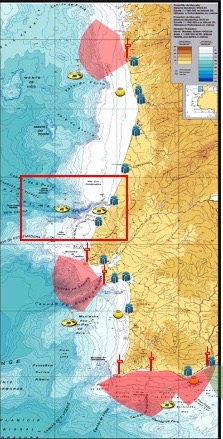
\includegraphics[scale=0.5]{fig/po-map.jpeg}}
  \hspace{+0.3cm} \subfigure[Zoomed in bathymetry showing the \naz
  canyon-Berlengas area (isobaths with depth in meters) and its
  environment including the placement of the two
  buoys.]{\label{fig:domain}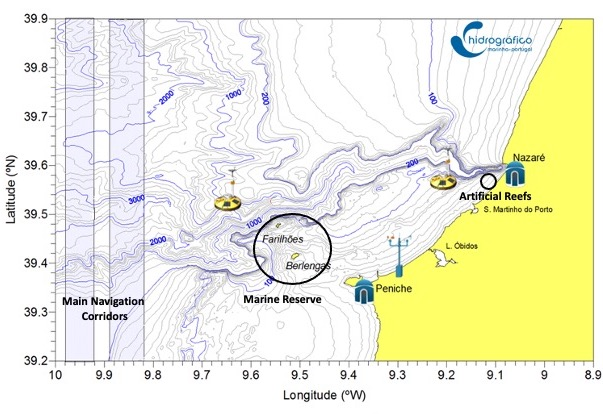
\includegraphics[scale=0.5]{fig/domain.jpg}}
  \subfigure[Predictions of currents and temperature at 10m depth from
  a \texttt{HOPS} (Harvard Ocean Prediction System) model with
  assimilation of temperature and salinity measurements collected by
  CTD profiles and
  current-meters.]{\label{fig:model}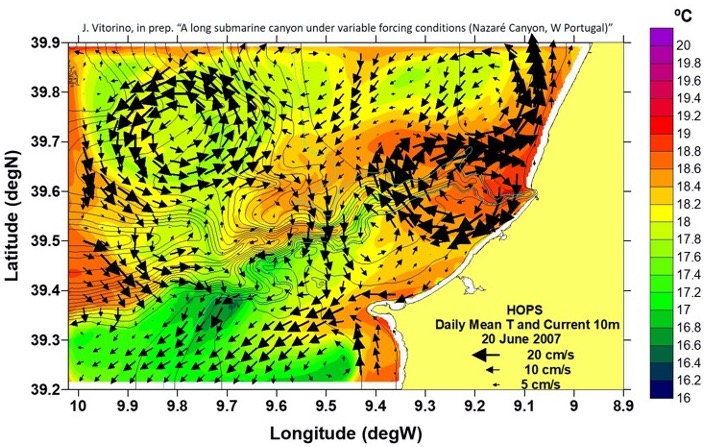
\includegraphics[scale=0.50]{fig/model.jpeg}}
  \caption{\subref{fig:po-map} \& \subref{fig:domain} show detailed
    views of the proposed study area for \proje, while
    \subref{fig:model} shows model predictions for the dynamic region
    driven by bathymetry and external forcing.}
  \label{fig:studyarea-1}
\end{figure}

\proj will focus on the area of influence of \naz Canyon located in
the central part of the western Portuguese coast and broadly extending
from 39.2ºN (south of Peniche) to 39.9 ºN (north of \naz)
(figure). This is a coastal ocean area well exposed to the influences
of the North Atlantic and marked by important topographic features
such as: the important changes of the continental margin associated
with the transition from the large Estremadura Plateau, in the
southern part , to the relatively narrow shelf north of \naz the
presence of a long and narrow submarine canyon, the \naz Canyon, that
extends for more than 200km from the head, just a few hundreds of
meters from the beach of \naze, incising the shelf into abyssal areas
the presence of island environments– the Berlengas Archipelago –
located a few tens of kilometers offshore the coast which is a
Natura2000 site recognized as a unique repository of genetic species
and habitat diversity on the western boundary of Europe and was
recently classified by UNESCO as Biosphere Reserve. The biogeographic,
geologic and oceanographic settings of this region, accentuated by the
presence of the \naz Canyon, are crucial for high levels of biological
productivity and biodiversity, induce dynamic ecological processes and
support many ecosystem services.  The \naz Canyon area of influence is
not directly impacted by major riverine outflows. The main rivers
influencing the western portuguese continental margin are the Douro
river (located at about 170 km to the north of \naze) and the Tagus
river (located at about 100 km to the south of \naze) with smaller
contributions from the Mondego river (50 km to the north of
\naze). During the winter and early spring the combined influence of
the Douro River and other smaller rivers such as the Mondego River
reach the \naz Canyon area during periods of northerly winds and
upwelling conditions, appearing as a low salinity water plume
occupying the first 30m of the water columns and extending over the
complete shelf as the result of offshore transport associated with the
prevailing upwelling conditions.  The influence of the Tagus River on
the area is less clear, largely due to the combination of the large
Estremadura Plateau with the shallow ridge between Cape Carvoeiro and
Berlegas areas and the associated circulation characteristics. Perhaps
more expressive for the conditions in the area is the contribution of
the small riverine sources that indent the \naze-Peniche coast during
periods of important precipitation. These include the contributions of
the small Alcoa and Tornadas rivers, of a large number of very small
fresh water courses (ribeiras) or from the Obidos Lagoon. Previous
observations showed that these contributions combine in a fresh and
high turbidity that can extend its influence over the complete shelf
(include photo) The seasonal evolution of wind forcing and wave
conditions that affect this area are largely determined by evolution
of the Azores High Pressure System. From May to September the Azores
High is typically located at northern positions, offshore the Iberian
Peninsula. The western Portuguese margin is then located on the
eastern branch of the High, under the influence of persistent
northerly winds (upwelling favorable) that during the summer months
are reinforced by the establishment of a thermal low over central
Iberia. The area is also protected from the influence of synoptic low
pressure systems, showing typically low energy swells (although
affected by locally generated seas associated with the sea breeze
circulation). During the winter months the conditions prevailing along
the western Portuguese margin are largely associated to the phase of
the winter North Atlantic Oscillation. During the negative phase of
the winter NAO the Azores High is typically located south of the
Iberian Peninsula and the western Portuguese coast is under the
influence of westerly and southwesterly qwind forcing that frequently
promote downwelling conditions and is exposed to the influence of
synoptic low pressure systems and an highly energetic wave
regime. During positive phases of the winter NAO the Azores High
remains at a high latitude leading to frequent periods of northerly
winds and upwelling conditions. During those periods the area is
largely protected from the influence of swells generated in the North
Atlantic.
 
 
Tidal motions on the are dominated by the semidiurnal lunar constituent
although in the large and shallow Estremadura plateau, in the south of
the area, Tidal currents over the shelf are generally of moderate
expression with speeds up to based on curremeters moorings and bottom
mounted ADCPs.  Much larges tidal motions are observed are near bottom
depths Inside the \naz Canyon, as the result of bottom focusing of
internal tide energy generated at the canyon rim.  along . Tidal the
 
The interaction of the barotropic tide with the shelf edge topography
in the presence of stratification opens the potential for generation
of internal tidal motions that propagate offshore to the deep ocean
domain and, if the stratification conditions if the continental shelf
allow, also onshore. The effect of these internal motions generated at
the shelf edge however remains, the waves being dissipated before
reaching the inner shelf environment. The major topography of \naz
Canyon however allows that internal tidal motions can be generated in
positions along the canyon rim to very close to the shore. Quaresma et
al. for example showed the expression and impact of solitons generated
close and that propagate towards the inner continental shelf impacting
the nutrient fluxes to the photic layer and the near bottom
sedimentary cover

